\documentclass[tikz, varwidth=600pt]{standalone}
\usepackage{amssymb, amsmath,bbm}

\standaloneenv{aaaa}

\begin{document}
	\begin{aaaa}
		\begin{center}	
		\fbox{%
			\begin{minipage}{0.85\linewidth}
				\centering
				\tikzset{every picture/.style={line width=0.75pt}} %set default line width to 0.75pt        
				\vspace{6pt} 
		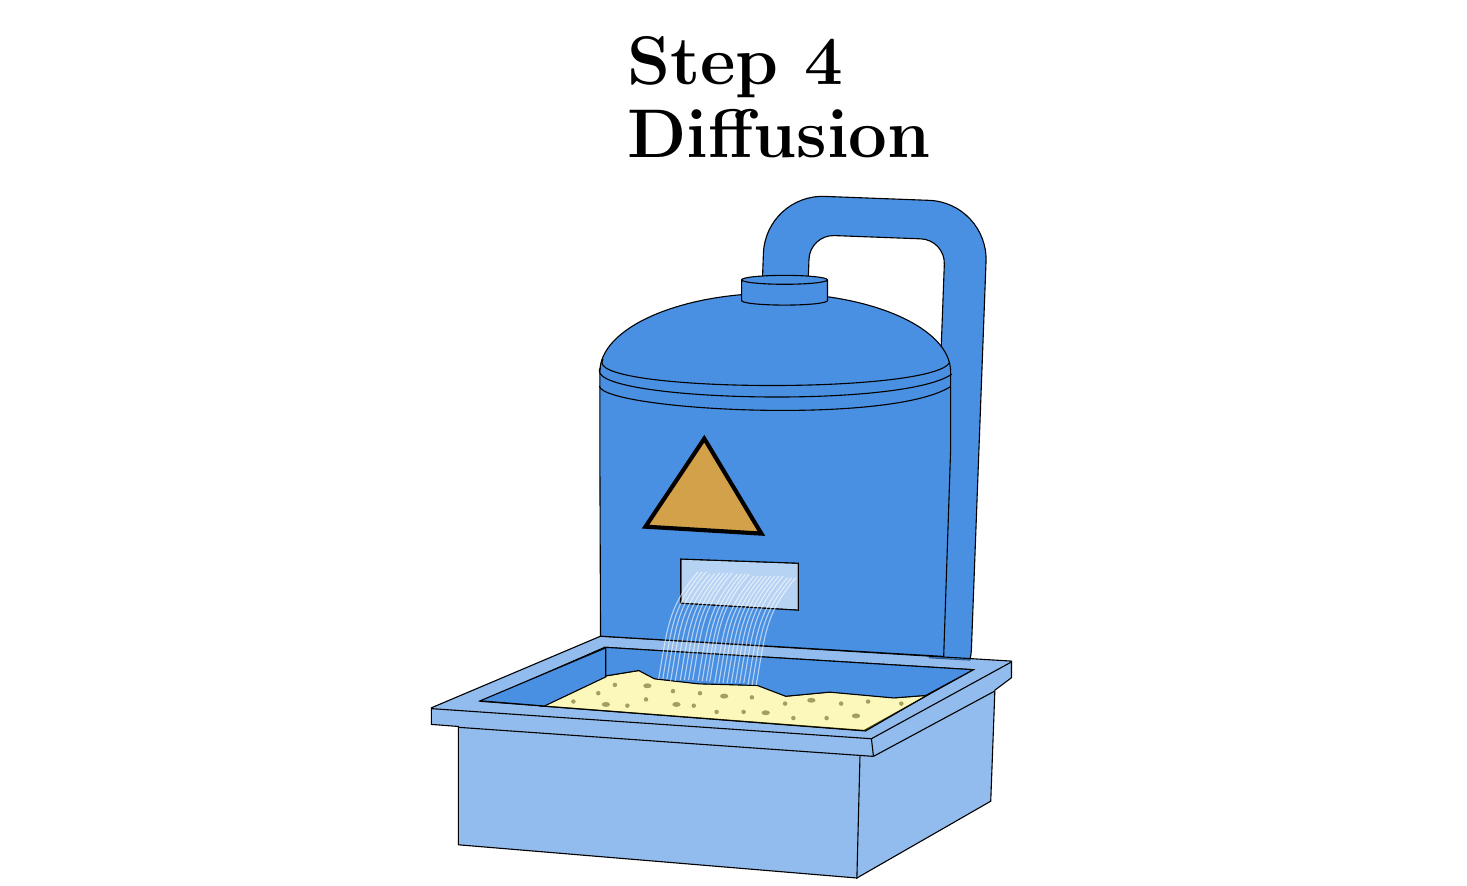
\begin{tikzpicture}[x=0.75pt,y=0.75pt,yscale=-1,xscale=1]
			%uncomment if require: \path (0,471); %set diagram left start at 0, and has height of 471
			    \path[use as bounding box] (0,0) rectangle (680,400);
			\begin{scope}[xshift=120pt,yshift=-5pt]
			%Shape: Polygon [id:ds4064514405975208] 
			\draw  [fill={rgb, 255:red, 74; green, 144; blue, 226 }  ,fill opacity=0.4 ] (211.33,287.33) -- (154.67,284) -- (154.67,262.67) -- (211.33,264.67) -- cycle ;
			%Shape: Path Data [id:dp35119156762297865] 
			\draw  [fill={rgb, 255:red, 74; green, 144; blue, 226 }  ,fill opacity=1 ] (224.01,87.96) -- (274.35,89.86) .. controls (290.06,90.45) and (302.33,103.68) .. (301.73,119.39) -- (294.7,305.83) .. controls (294.63,307.73) and (294.37,309.58) .. (293.95,311.36) -- (274.49,310.26) -- (281.64,120.64) .. controls (281.89,114.13) and (276.81,108.66) .. (270.3,108.41) -- (228.67,106.84) .. controls (222.16,106.6) and (216.68,111.67) .. (216.44,118.18) -- (215.43,144.86) -- (193.39,144.22) -- (194.48,115.35) .. controls (195.07,99.63) and (208.29,87.37) .. (224.01,87.96) -- cycle ;
			%Shape: Polygon [id:ds8510150227056082] 
			\draw  [fill={rgb, 255:red, 74; green, 144; blue, 226 }  ,fill opacity=0.6 ] (304,379.35) -- (239.5,416.35) -- (47.5,400.35) -- (47.5,343.35) -- (34.5,342.35) -- (34.5,334.35) -- (116,299.85) -- (314,311.85) -- (314,319.85) -- (306,325.85) -- cycle ;
			%Straight Lines [id:da3654938941022118] 
			\draw    (47.5,343.75) -- (247.5,357.75) ;
			%Straight Lines [id:da12503765856262283] 
			\draw    (247.5,357.75) -- (306,326.25) ;
			%Straight Lines [id:da5166787893395551] 
			\draw    (34.5,334.75) -- (246.5,349.25) ;
			%Straight Lines [id:da9333334976241038] 
			\draw    (246.5,349.25) -- (314,312.25) ;
			%Straight Lines [id:da998347705627445] 
			\draw    (246.5,349.25) -- (247.5,357.75) ;
			%Straight Lines [id:da6909125343637312] 
			\draw [fill={rgb, 255:red, 74; green, 144; blue, 226 }  ,fill opacity=1 ]   (239.5,416.75) -- (241,357.75) ;
			%Shape: Path Data [id:dp22686871453193025] 
			\draw  [fill={rgb, 255:red, 74; green, 144; blue, 226 }  ,fill opacity=1 ] (115.67,172.43) .. controls (115.67,151.54) and (153.5,134.6) .. (200.17,134.6) .. controls (246.83,134.6) and (284.67,151.54) .. (284.67,172.43) -- (284.67,210.27) -- (281.33,309.6) -- (116,299.85) -- (115.67,210.27) -- (115.67,172.43) -- cycle (211.33,287.33) -- (211.33,264.67) -- (154.67,262.67) -- (154.67,284) -- (211.33,287.33) -- cycle ;
			%Shape: Polygon [id:ds6961869257044322] 
			\draw  [fill={rgb, 255:red, 245; green, 166; blue, 35 }  ,fill opacity=0.8 ][line width=1.5]  (166,204.67) -- (193.5,250.42) -- (137.67,247.08) -- cycle ;
			%Curve Lines [id:da6943308282030407] 
			\draw    (115.4,179.4) .. controls (118,191) and (255.2,198.4) .. (284.6,179.6) ;
			%Curve Lines [id:da6433057190127286] 
			\draw    (116,170.4) .. controls (104.6,186.4) and (260.8,190.8) .. (285.2,173.6) ;
			%Curve Lines [id:da9012210298300685] 
			\draw    (117.2,166.4) .. controls (105.8,182.4) and (275.2,183.6) .. (284.2,168) ;
			%Shape: Polygon [id:ds37127469012501024] 
			\draw   (243,345.25) -- (86.8,333.2) -- (117.2,318.8) -- (134.4,316) -- (142,320) -- (163.2,322.4) -- (191.6,323.2) -- (205.2,328.4) -- (226.4,326.4) -- (257.2,329.2) -- (272.8,328) -- cycle ;
			%Shape: Polygon [id:ds5590572248497979] 
			\draw  [fill={rgb, 255:red, 255; green, 255; blue, 255 }  ,fill opacity=1 ] (243,345.25) -- (58.5,331.25) -- (118,305.2) -- (295.6,316) -- cycle ;
			%Shape: Circle [id:dp39275733445484073] 
			\draw  [draw opacity=0][fill={rgb, 255:red, 0; green, 0; blue, 0 }  ,fill opacity=0.5 ] (101.83,331.32) .. controls (101.83,330.72) and (102.32,330.23) .. (102.92,330.23) .. controls (103.51,330.23) and (104,330.72) .. (104,331.32) .. controls (104,331.92) and (103.51,332.4) .. (102.92,332.4) .. controls (102.32,332.4) and (101.83,331.92) .. (101.83,331.32) -- cycle ;
			%Shape: Ellipse [id:dp31448593349952836] 
			\draw  [draw opacity=0][fill={rgb, 255:red, 0; green, 0; blue, 0 }  ,fill opacity=0.5 ] (116.58,332.73) .. controls (116.58,332.07) and (117.48,331.54) .. (118.58,331.54) .. controls (119.69,331.54) and (120.58,332.07) .. (120.58,332.73) .. controls (120.58,333.39) and (119.69,333.92) .. (118.58,333.92) .. controls (117.48,333.92) and (116.58,333.39) .. (116.58,332.73) -- cycle ;
			%Shape: Ellipse [id:dp35150330418693454] 
			\draw  [draw opacity=0][fill={rgb, 255:red, 0; green, 0; blue, 0 }  ,fill opacity=0.5 ] (237.08,338.23) .. controls (237.08,337.57) and (237.98,337.04) .. (239.08,337.04) .. controls (240.19,337.04) and (241.08,337.57) .. (241.08,338.23) .. controls (241.08,338.89) and (240.19,339.42) .. (239.08,339.42) .. controls (237.98,339.42) and (237.08,338.89) .. (237.08,338.23) -- cycle ;
			%Shape: Ellipse [id:dp49355274026905915] 
			\draw  [draw opacity=0][fill={rgb, 255:red, 0; green, 0; blue, 0 }  ,fill opacity=0.5 ] (136.58,323.73) .. controls (136.58,323.07) and (137.48,322.54) .. (138.58,322.54) .. controls (139.69,322.54) and (140.58,323.07) .. (140.58,323.73) .. controls (140.58,324.39) and (139.69,324.92) .. (138.58,324.92) .. controls (137.48,324.92) and (136.58,324.39) .. (136.58,323.73) -- cycle ;
			%Shape: Ellipse [id:dp24462867957943346] 
			\draw  [draw opacity=0][fill={rgb, 255:red, 0; green, 0; blue, 0 }  ,fill opacity=0.5 ] (150.58,332.73) .. controls (150.58,332.07) and (151.48,331.54) .. (152.58,331.54) .. controls (153.69,331.54) and (154.58,332.07) .. (154.58,332.73) .. controls (154.58,333.39) and (153.69,333.92) .. (152.58,333.92) .. controls (151.48,333.92) and (150.58,333.39) .. (150.58,332.73) -- cycle ;
			%Shape: Ellipse [id:dp37076534245874304] 
			\draw  [draw opacity=0][fill={rgb, 255:red, 0; green, 0; blue, 0 }  ,fill opacity=0.5 ] (173.58,328.73) .. controls (173.58,328.07) and (174.48,327.54) .. (175.58,327.54) .. controls (176.69,327.54) and (177.58,328.07) .. (177.58,328.73) .. controls (177.58,329.39) and (176.69,329.92) .. (175.58,329.92) .. controls (174.48,329.92) and (173.58,329.39) .. (173.58,328.73) -- cycle ;
			%Shape: Ellipse [id:dp0958160725182382] 
			\draw  [draw opacity=0][fill={rgb, 255:red, 0; green, 0; blue, 0 }  ,fill opacity=0.5 ] (193.58,336.73) .. controls (193.58,336.07) and (194.48,335.54) .. (195.58,335.54) .. controls (196.69,335.54) and (197.58,336.07) .. (197.58,336.73) .. controls (197.58,337.39) and (196.69,337.92) .. (195.58,337.92) .. controls (194.48,337.92) and (193.58,337.39) .. (193.58,336.73) -- cycle ;
			%Shape: Ellipse [id:dp346353664426017] 
			\draw  [draw opacity=0][fill={rgb, 255:red, 0; green, 0; blue, 0 }  ,fill opacity=0.5 ] (215.58,330.73) .. controls (215.58,330.07) and (216.48,329.54) .. (217.58,329.54) .. controls (218.69,329.54) and (219.58,330.07) .. (219.58,330.73) .. controls (219.58,331.39) and (218.69,331.92) .. (217.58,331.92) .. controls (216.48,331.92) and (215.58,331.39) .. (215.58,330.73) -- cycle ;
			%Shape: Circle [id:dp10529033599899029] 
			\draw  [draw opacity=0][fill={rgb, 255:red, 0; green, 0; blue, 0 }  ,fill opacity=0.5 ] (121.83,323.32) .. controls (121.83,322.72) and (122.32,322.23) .. (122.92,322.23) .. controls (123.51,322.23) and (124,322.72) .. (124,323.32) .. controls (124,323.92) and (123.51,324.4) .. (122.92,324.4) .. controls (122.32,324.4) and (121.83,323.92) .. (121.83,323.32) -- cycle ;
			%Shape: Circle [id:dp6006715128229848] 
			\draw  [draw opacity=0][fill={rgb, 255:red, 0; green, 0; blue, 0 }  ,fill opacity=0.5 ] (113.83,327.32) .. controls (113.83,326.72) and (114.32,326.23) .. (114.92,326.23) .. controls (115.51,326.23) and (116,326.72) .. (116,327.32) .. controls (116,327.92) and (115.51,328.4) .. (114.92,328.4) .. controls (114.32,328.4) and (113.83,327.92) .. (113.83,327.32) -- cycle ;
			%Shape: Circle [id:dp8376114765926564] 
			\draw  [draw opacity=0][fill={rgb, 255:red, 0; green, 0; blue, 0 }  ,fill opacity=0.5 ] (127.83,333.32) .. controls (127.83,332.72) and (128.32,332.23) .. (128.92,332.23) .. controls (129.51,332.23) and (130,332.72) .. (130,333.32) .. controls (130,333.92) and (129.51,334.4) .. (128.92,334.4) .. controls (128.32,334.4) and (127.83,333.92) .. (127.83,333.32) -- cycle ;
			%Shape: Circle [id:dp9731363908931567] 
			\draw  [draw opacity=0][fill={rgb, 255:red, 0; green, 0; blue, 0 }  ,fill opacity=0.5 ] (136.83,330.32) .. controls (136.83,329.72) and (137.32,329.23) .. (137.92,329.23) .. controls (138.51,329.23) and (139,329.72) .. (139,330.32) .. controls (139,330.92) and (138.51,331.4) .. (137.92,331.4) .. controls (137.32,331.4) and (136.83,330.92) .. (136.83,330.32) -- cycle ;
			%Shape: Circle [id:dp6457093405767959] 
			\draw  [draw opacity=0][fill={rgb, 255:red, 0; green, 0; blue, 0 }  ,fill opacity=0.5 ] (149.83,326.32) .. controls (149.83,325.72) and (150.32,325.23) .. (150.92,325.23) .. controls (151.51,325.23) and (152,325.72) .. (152,326.32) .. controls (152,326.92) and (151.51,327.4) .. (150.92,327.4) .. controls (150.32,327.4) and (149.83,326.92) .. (149.83,326.32) -- cycle ;
			%Shape: Circle [id:dp4916349805601372] 
			\draw  [draw opacity=0][fill={rgb, 255:red, 0; green, 0; blue, 0 }  ,fill opacity=0.5 ] (159.83,333.32) .. controls (159.83,332.72) and (160.32,332.23) .. (160.92,332.23) .. controls (161.51,332.23) and (162,332.72) .. (162,333.32) .. controls (162,333.92) and (161.51,334.4) .. (160.92,334.4) .. controls (160.32,334.4) and (159.83,333.92) .. (159.83,333.32) -- cycle ;
			%Shape: Circle [id:dp12500273836257447] 
			\draw  [draw opacity=0][fill={rgb, 255:red, 0; green, 0; blue, 0 }  ,fill opacity=0.5 ] (162.83,327.32) .. controls (162.83,326.72) and (163.32,326.23) .. (163.92,326.23) .. controls (164.51,326.23) and (165,326.72) .. (165,327.32) .. controls (165,327.92) and (164.51,328.4) .. (163.92,328.4) .. controls (163.32,328.4) and (162.83,327.92) .. (162.83,327.32) -- cycle ;
			%Shape: Circle [id:dp7128068113839312] 
			\draw  [draw opacity=0][fill={rgb, 255:red, 0; green, 0; blue, 0 }  ,fill opacity=0.5 ] (170.83,336.32) .. controls (170.83,335.72) and (171.32,335.23) .. (171.92,335.23) .. controls (172.51,335.23) and (173,335.72) .. (173,336.32) .. controls (173,336.92) and (172.51,337.4) .. (171.92,337.4) .. controls (171.32,337.4) and (170.83,336.92) .. (170.83,336.32) -- cycle ;
			%Shape: Circle [id:dp9742134134811231] 
			\draw  [draw opacity=0][fill={rgb, 255:red, 0; green, 0; blue, 0 }  ,fill opacity=0.5 ] (183.83,336.32) .. controls (183.83,335.72) and (184.32,335.23) .. (184.92,335.23) .. controls (185.51,335.23) and (186,335.72) .. (186,336.32) .. controls (186,336.92) and (185.51,337.4) .. (184.92,337.4) .. controls (184.32,337.4) and (183.83,336.92) .. (183.83,336.32) -- cycle ;
			%Shape: Circle [id:dp26816404412020256] 
			\draw  [draw opacity=0][fill={rgb, 255:red, 0; green, 0; blue, 0 }  ,fill opacity=0.5 ] (187.83,329.32) .. controls (187.83,328.72) and (188.32,328.23) .. (188.92,328.23) .. controls (189.51,328.23) and (190,328.72) .. (190,329.32) .. controls (190,329.92) and (189.51,330.4) .. (188.92,330.4) .. controls (188.32,330.4) and (187.83,329.92) .. (187.83,329.32) -- cycle ;
			%Shape: Circle [id:dp42256651163442593] 
			\draw  [draw opacity=0][fill={rgb, 255:red, 0; green, 0; blue, 0 }  ,fill opacity=0.5 ] (207.83,339.32) .. controls (207.83,338.72) and (208.32,338.23) .. (208.92,338.23) .. controls (209.51,338.23) and (210,338.72) .. (210,339.32) .. controls (210,339.92) and (209.51,340.4) .. (208.92,340.4) .. controls (208.32,340.4) and (207.83,339.92) .. (207.83,339.32) -- cycle ;
			%Shape: Circle [id:dp10842289928900717] 
			\draw  [draw opacity=0][fill={rgb, 255:red, 0; green, 0; blue, 0 }  ,fill opacity=0.5 ] (203.83,332.32) .. controls (203.83,331.72) and (204.32,331.23) .. (204.92,331.23) .. controls (205.51,331.23) and (206,331.72) .. (206,332.32) .. controls (206,332.92) and (205.51,333.4) .. (204.92,333.4) .. controls (204.32,333.4) and (203.83,332.92) .. (203.83,332.32) -- cycle ;
			%Shape: Circle [id:dp46917832640043966] 
			\draw  [draw opacity=0][fill={rgb, 255:red, 0; green, 0; blue, 0 }  ,fill opacity=0.5 ] (223.83,339.32) .. controls (223.83,338.72) and (224.32,338.23) .. (224.92,338.23) .. controls (225.51,338.23) and (226,338.72) .. (226,339.32) .. controls (226,339.92) and (225.51,340.4) .. (224.92,340.4) .. controls (224.32,340.4) and (223.83,339.92) .. (223.83,339.32) -- cycle ;
			%Shape: Circle [id:dp37636578246789687] 
			\draw  [draw opacity=0][fill={rgb, 255:red, 0; green, 0; blue, 0 }  ,fill opacity=0.5 ] (243.83,331.32) .. controls (243.83,330.72) and (244.32,330.23) .. (244.92,330.23) .. controls (245.51,330.23) and (246,330.72) .. (246,331.32) .. controls (246,331.92) and (245.51,332.4) .. (244.92,332.4) .. controls (244.32,332.4) and (243.83,331.92) .. (243.83,331.32) -- cycle ;
			%Shape: Circle [id:dp7395819002133621] 
			\draw  [draw opacity=0][fill={rgb, 255:red, 0; green, 0; blue, 0 }  ,fill opacity=0.5 ] (259.83,332.32) .. controls (259.83,331.72) and (260.32,331.23) .. (260.92,331.23) .. controls (261.51,331.23) and (262,331.72) .. (262,332.32) .. controls (262,332.92) and (261.51,333.4) .. (260.92,333.4) .. controls (260.32,333.4) and (259.83,332.92) .. (259.83,332.32) -- cycle ;
			%Shape: Circle [id:dp04074607388341378] 
			\draw  [draw opacity=0][fill={rgb, 255:red, 0; green, 0; blue, 0 }  ,fill opacity=0.5 ] (230.83,332.32) .. controls (230.83,331.72) and (231.32,331.23) .. (231.92,331.23) .. controls (232.51,331.23) and (233,331.72) .. (233,332.32) .. controls (233,332.92) and (232.51,333.4) .. (231.92,333.4) .. controls (231.32,333.4) and (230.83,332.92) .. (230.83,332.32) -- cycle ;
			%Shape: Polygon [id:ds7403641988997934] 
			\draw  [fill={rgb, 255:red, 248; green, 231; blue, 28 }  ,fill opacity=0.3 ] (243.63,345.52) -- (87.43,333.47) -- (117.83,319.07) -- (135.03,316.27) -- (142.63,320.27) -- (163.83,322.67) -- (192.23,323.47) -- (205.83,328.67) -- (227.03,326.67) -- (257.83,329.47) -- (273.43,328.27) -- cycle ;
			
			%Shape: Path Data [id:dp15167970180235957] 
			\draw  [fill={rgb, 255:red, 74; green, 144; blue, 226 }  ,fill opacity=1 ] (118,305.2) -- (295.6,316) -- (272.68,328.41) -- (257.2,329.6) -- (226.4,326.8) -- (205.2,328.8) -- (191.6,323.6) -- (163.2,322.8) -- (142,320.4) -- (134.4,316.4) -- (117.33,319.18) -- (118,305.2) -- cycle ;
			%Shape: Can [id:dp5313849140147021] 
			\draw  [fill={rgb, 255:red, 74; green, 144; blue, 226 }  ,fill opacity=1 ] (225.33,128.15) -- (225.33,138.18) .. controls (225.33,139.37) and (216.08,140.33) .. (204.67,140.33) .. controls (193.25,140.33) and (184,139.37) .. (184,138.18) -- (184,128.15) .. controls (184,126.96) and (193.25,126) .. (204.67,126) .. controls (216.08,126) and (225.33,126.96) .. (225.33,128.15) .. controls (225.33,129.34) and (216.08,130.3) .. (204.67,130.3) .. controls (193.25,130.3) and (184,129.34) .. (184,128.15) ;
			%Curve Lines [id:da11890683366170429] 
			\draw [color={rgb, 255:red, 255; green, 255; blue, 255 }  ,draw opacity=0.6 ]   (163,268.8) .. controls (148.8,285.6) and (148.4,294.8) .. (144,320.4) ;
			%Curve Lines [id:da6407453953597059] 
			\draw [color={rgb, 255:red, 255; green, 255; blue, 255 }  ,draw opacity=0.6 ]   (165,268.8) .. controls (150.8,285.6) and (150.4,294.8) .. (146,320.4) ;
			%Curve Lines [id:da16506423302123296] 
			\draw [color={rgb, 255:red, 255; green, 255; blue, 255 }  ,draw opacity=0.6 ]   (167,268.8) .. controls (152.8,285.6) and (152.4,294.8) .. (148,320.4) ;
			%Curve Lines [id:da9514382268865446] 
			\draw [color={rgb, 255:red, 255; green, 255; blue, 255 }  ,draw opacity=0.6 ]   (168.78,269.8) .. controls (154.58,286.6) and (154.18,295.8) .. (149.78,321.4) ;
			%Curve Lines [id:da2567602694986312] 
			\draw [color={rgb, 255:red, 255; green, 255; blue, 255 }  ,draw opacity=0.6 ]   (171,269.8) .. controls (156.8,286.6) and (156.4,295.8) .. (152,321.4) ;
			%Curve Lines [id:da05920584738558232] 
			\draw [color={rgb, 255:red, 255; green, 255; blue, 255 }  ,draw opacity=0.6 ]   (173.4,269.4) .. controls (159.2,286.2) and (158.8,295.4) .. (154.4,321) ;
			%Curve Lines [id:da2900942609843956] 
			\draw [color={rgb, 255:red, 255; green, 255; blue, 255 }  ,draw opacity=0.6 ]   (175.4,269.4) .. controls (161.2,286.2) and (160.8,295.4) .. (156.4,321) ;
			%Curve Lines [id:da23451953818375448] 
			\draw [color={rgb, 255:red, 255; green, 255; blue, 255 }  ,draw opacity=0.6 ]   (177.4,269.4) .. controls (163.2,286.2) and (162.8,295.4) .. (158.4,321) ;
			%Curve Lines [id:da5811681610315563] 
			\draw [color={rgb, 255:red, 255; green, 255; blue, 255 }  ,draw opacity=0.6 ]   (179.4,269.4) .. controls (165.2,286.2) and (164.8,295.4) .. (160.4,321) ;
			%Curve Lines [id:da9402256005421262] 
			\draw [color={rgb, 255:red, 255; green, 255; blue, 255 }  ,draw opacity=0.6 ]   (182,269.8) .. controls (167.8,286.6) and (167.4,295.8) .. (163,321.4) ;
			%Curve Lines [id:da5764797473447335] 
			\draw [color={rgb, 255:red, 255; green, 255; blue, 255 }  ,draw opacity=0.6 ]   (184,269.8) .. controls (169.8,286.6) and (169.4,295.8) .. (165,321.4) ;
			%Curve Lines [id:da38140809653388486] 
			\draw [color={rgb, 255:red, 255; green, 255; blue, 255 }  ,draw opacity=0.6 ]   (186,269.8) .. controls (171.8,286.6) and (171.4,295.8) .. (167,321.4) ;
			%Curve Lines [id:da7302677970246141] 
			\draw [color={rgb, 255:red, 255; green, 255; blue, 255 }  ,draw opacity=0.6 ]   (187.6,270) .. controls (173.4,286.8) and (173,296) .. (168.6,321.6) ;
			%Curve Lines [id:da26833662389498014] 
			\draw [color={rgb, 255:red, 255; green, 255; blue, 255 }  ,draw opacity=0.6 ]   (190,270.8) .. controls (175.8,287.6) and (175.4,296.8) .. (171,322.4) ;
			%Curve Lines [id:da8034948507944907] 
			\draw [color={rgb, 255:red, 255; green, 255; blue, 255 }  ,draw opacity=0.6 ]   (192,270.8) .. controls (177.8,287.6) and (177.4,296.8) .. (173,322.4) ;
			%Curve Lines [id:da6322672557369288] 
			\draw [color={rgb, 255:red, 255; green, 255; blue, 255 }  ,draw opacity=0.6 ]   (194,270.8) .. controls (179.8,287.6) and (179.4,296.8) .. (175,322.4) ;
			%Curve Lines [id:da6446209891733293] 
			\draw [color={rgb, 255:red, 255; green, 255; blue, 255 }  ,draw opacity=0.6 ]   (196,270.8) .. controls (181.8,287.6) and (181.4,296.8) .. (177,322.4) ;
			%Curve Lines [id:da033700031234834116] 
			\draw [color={rgb, 255:red, 255; green, 255; blue, 255 }  ,draw opacity=0.6 ]   (198,270.8) .. controls (183.8,287.6) and (183.4,296.8) .. (179,322.4) ;
			%Curve Lines [id:da49289972726629216] 
			\draw [color={rgb, 255:red, 255; green, 255; blue, 255 }  ,draw opacity=0.6 ]   (200,270.8) .. controls (185.8,287.6) and (185.4,296.8) .. (181,322.4) ;
			%Curve Lines [id:da025876931878601073] 
			\draw [color={rgb, 255:red, 255; green, 255; blue, 255 }  ,draw opacity=0.6 ]   (202,270.8) .. controls (187.8,287.6) and (187.4,296.8) .. (183,322.4) ;
			%Curve Lines [id:da37977946993571066] 
			\draw [color={rgb, 255:red, 255; green, 255; blue, 255 }  ,draw opacity=0.6 ]   (204,270.8) .. controls (189.8,287.6) and (189.4,296.8) .. (185,322.4) ;
			%Curve Lines [id:da17883227814698366] 
			\draw [color={rgb, 255:red, 255; green, 255; blue, 255 }  ,draw opacity=0.6 ]   (206,271.8) .. controls (191.8,288.6) and (191.4,297.8) .. (187,323.4) ;
			%Curve Lines [id:da44782467334225184] 
			\draw [color={rgb, 255:red, 255; green, 255; blue, 255 }  ,draw opacity=0.6 ]   (208,271.8) .. controls (193.8,288.6) and (193.4,297.8) .. (189,323.4) ;
			%Curve Lines [id:da9754395069705338] 
			\draw [color={rgb, 255:red, 255; green, 255; blue, 255 }  ,draw opacity=0.6 ]   (210,271.8) .. controls (195.8,288.6) and (195.4,297.8) .. (191,323.4) ;
			%Shape: Polygon [id:ds644624856146738] 
			\draw  [fill={rgb, 255:red, 74; green, 144; blue, 226 }  ,fill opacity=1 ] (118.5,305.48) -- (118.5,319.48) -- (89,333.48) -- (58,330.98) -- cycle ;
			
			% Text Node
			\draw (127.67,45) node [anchor=north west][inner sep=0.75pt]  [font=\Huge] [align=left] {\textbf{Diffusion}};
			
			% Text Node
			\draw (127.67,10) node [anchor=north west][inner sep=0.75pt]  [font=\Huge] [align=left] {\textbf{Step 4}};
			\end{scope}
		\end{tikzpicture}
	
		\vspace{6pt}
		\end{minipage}}
		\end{center}
	\end{aaaa}
\end{document}